\section{Konsole}
\label{sec:Konsole}
\subsection{Training}
\label{sec:Training}
\subsubsection{Input}
\label{sec:TraiInput}
\begin{lstlisting}[language=bash]
ki --training "[trainings.ubyte]"
\end{lstlisting}

\subsubsection{Output}
\label{sec:TraiOutput}
Nach jedem Datensatz wird angezeigt, wie viele der zum Training gegebenen Daten bereits abgearbeitet wurden. 

\subsection{Test}
\label{sec:Test}
\subsubsection{Input}
\label{sec:TestInput}
\begin{lstlisting}[language=bash]
ki --test "[test.ubyte]"
\end{lstlisting}

\subsubsection{Output}
\label{sec:TestOutput}
Nach jedem Datensatz wird angezeigt, wie viele der zum Testen gegebenen Daten bereits abgearbeitet wurden. Zudem wird angezeigt, wie viele der Datensatz richtig bzw. falsch erkannt wurden.



\subsection{Anwendung}
\label{sec:Anwendung}
\subsubsection{Input}
\label{sec:UseInput}
\begin{lstlisting}[language=bash]
ki "[image.jpg]"
\end{lstlisting}

\subsubsection{Output}
\label{sec:UseOutput}
Als Output werden alle Ziffern von 0 bis 9 mit den entsprechenden Prozentwerten zur�ckgegeben (Dies kommt daher, dass die KI die Wahrscheinlichkeit der �bereinstimmung f�r jede Ziffer berechnet.). Zudem wird auch angezeigt, welche Ziffer die h�chste �bereinstimmung hat. Da diese die erkannte Ziffer darstellt.

\section{Datenbank}
\label{sec:Datenbank}
Die Applikation ben�tigt keine Datenbank.

\section{Code}
\label{sec:Code}
\subsection{Klassendiagramm}
\label{sec:Klassendiagramm}
 Es gibt drei Klassen in CKi (Convolutional Layer, Pooling Layer, Dense Layers). Ein Convolutional Layer ist eine Art von Filter, welcher auf das Bild gelegt wird, um eine vereinfachte Erkennung zu erm�glichen. Die Pooling Layers sind verantwortlich das Bild zu verkleinern und so eine schnellere Verarbeitung zu erm�glichen. Die Dense Layers oder auch Fully Connected Layers sind das eigentlich das Gehirn der KI. Zus�tzlich gibt es die Main-Klasse, diese ist zust�ndig die oben genannten Klassen miteinander zu verbinden und so das Netzwerk aufzubauen. Zus�tzlich handhabt es die Nutzereingaben und die Auslese der Trainings-/Testdaten. 

\begin{figure}[H]
\centering
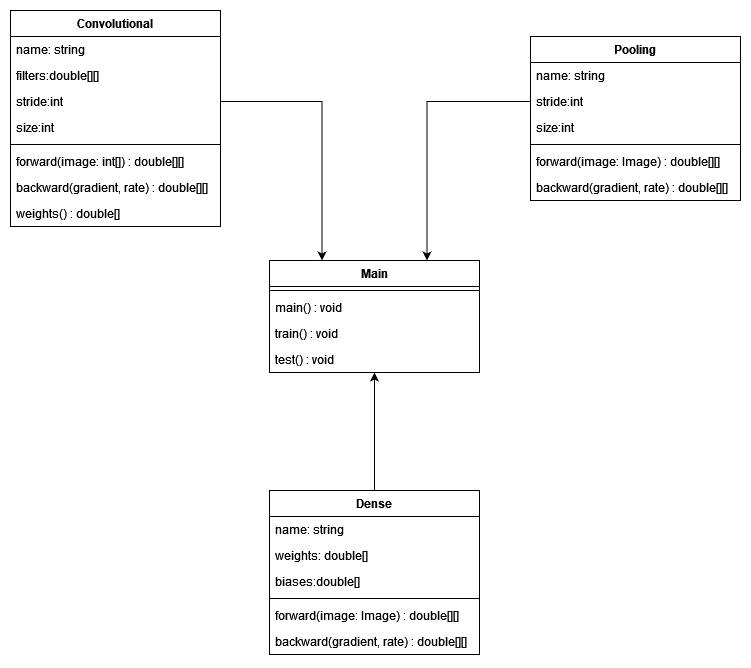
\includegraphics[height=0.5\paperheight]{Klassendiagramm.png}
\caption{Das Klassendiagramm, Grundaufbau der Applikation}
\label{fig:klassendiagramm}
\end{figure}

\subsection{Trainingsdaten}
\label{sec:Trainingsdaten}
Die Trainingsdaten sind das MNIST-Datenset mit den handschriftlichen Zahlen. (\url{http://yann.lecun.com/exdb/mnist/})

\subsection{Tests}
\label{sec:Tests}

